\chapter{PENDAHULUAN}

\section{Latar Belakang}
Seni melipat kertas, atau origami, telah berkembang dari kerajinan tradisional menjadi objek studi ilmiah yang melibatkan matematika, ilmu komputer, dan rekayasa struktur. Secara matematis, seluruh lipatan pada kertas direpresentasikan melalui graf planar dua dimensi yang disebut pola lipatan (\textit{crease pattern}). Konstruksi geometri pelipatan ini diformalkan melalui aksioma kombinatorik ketat, seperti Aksioma Huzita-Hatori, yang mendefinisikan seluruh operasi dasar pelipatan yang mungkin dilakukan \parencite{hull2012project}.

Salah satu subbidang riset yang paling aplikatif adalah pelipatan kaku (\textit{rigid folding}). Pelipatan kaku memodelkan setiap panel kertas yang dibatasi oleh garis lipatan sebagai material tegar (benda kaku) yang tidak dapat ditekuk secara kontinu, melainkan hanya berputar secara kaku pada sumbu engsel lipatannya. Proses dinamika spasial dari kondisi kertas datar menuju kertas terlipat sempurna dapat divisualisasikan melalui tahapan pergerakan verteks, sebagaimana diilustrasikan pada \ref{fig:origami_stages}.

\begin{figure}[H]
  \centering
  \begin{minipage}{0.32\textwidth}
    \centering
    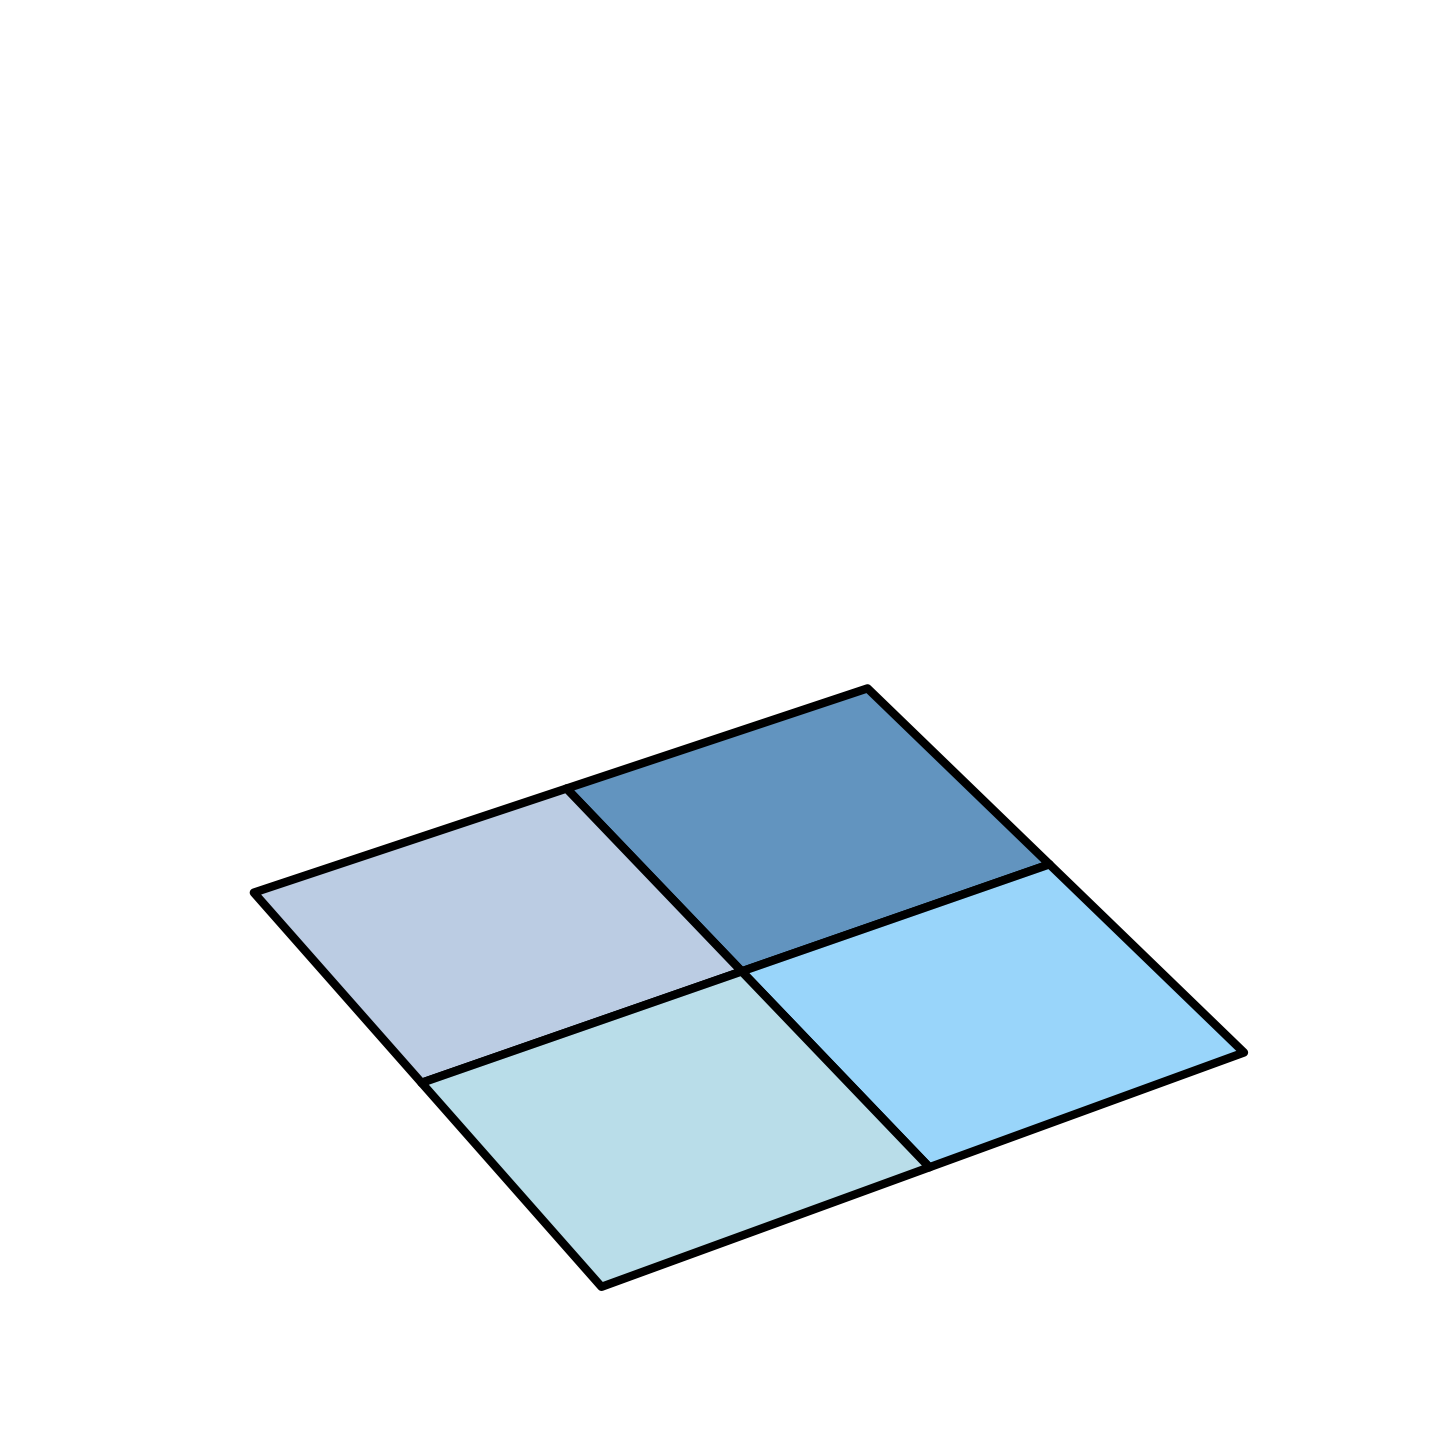
\includegraphics[width=\linewidth]{foto/origami_stage1.png}
    (a) Fase Datar
  \end{minipage}\hfill
  \begin{minipage}{0.32\textwidth}
    \centering
    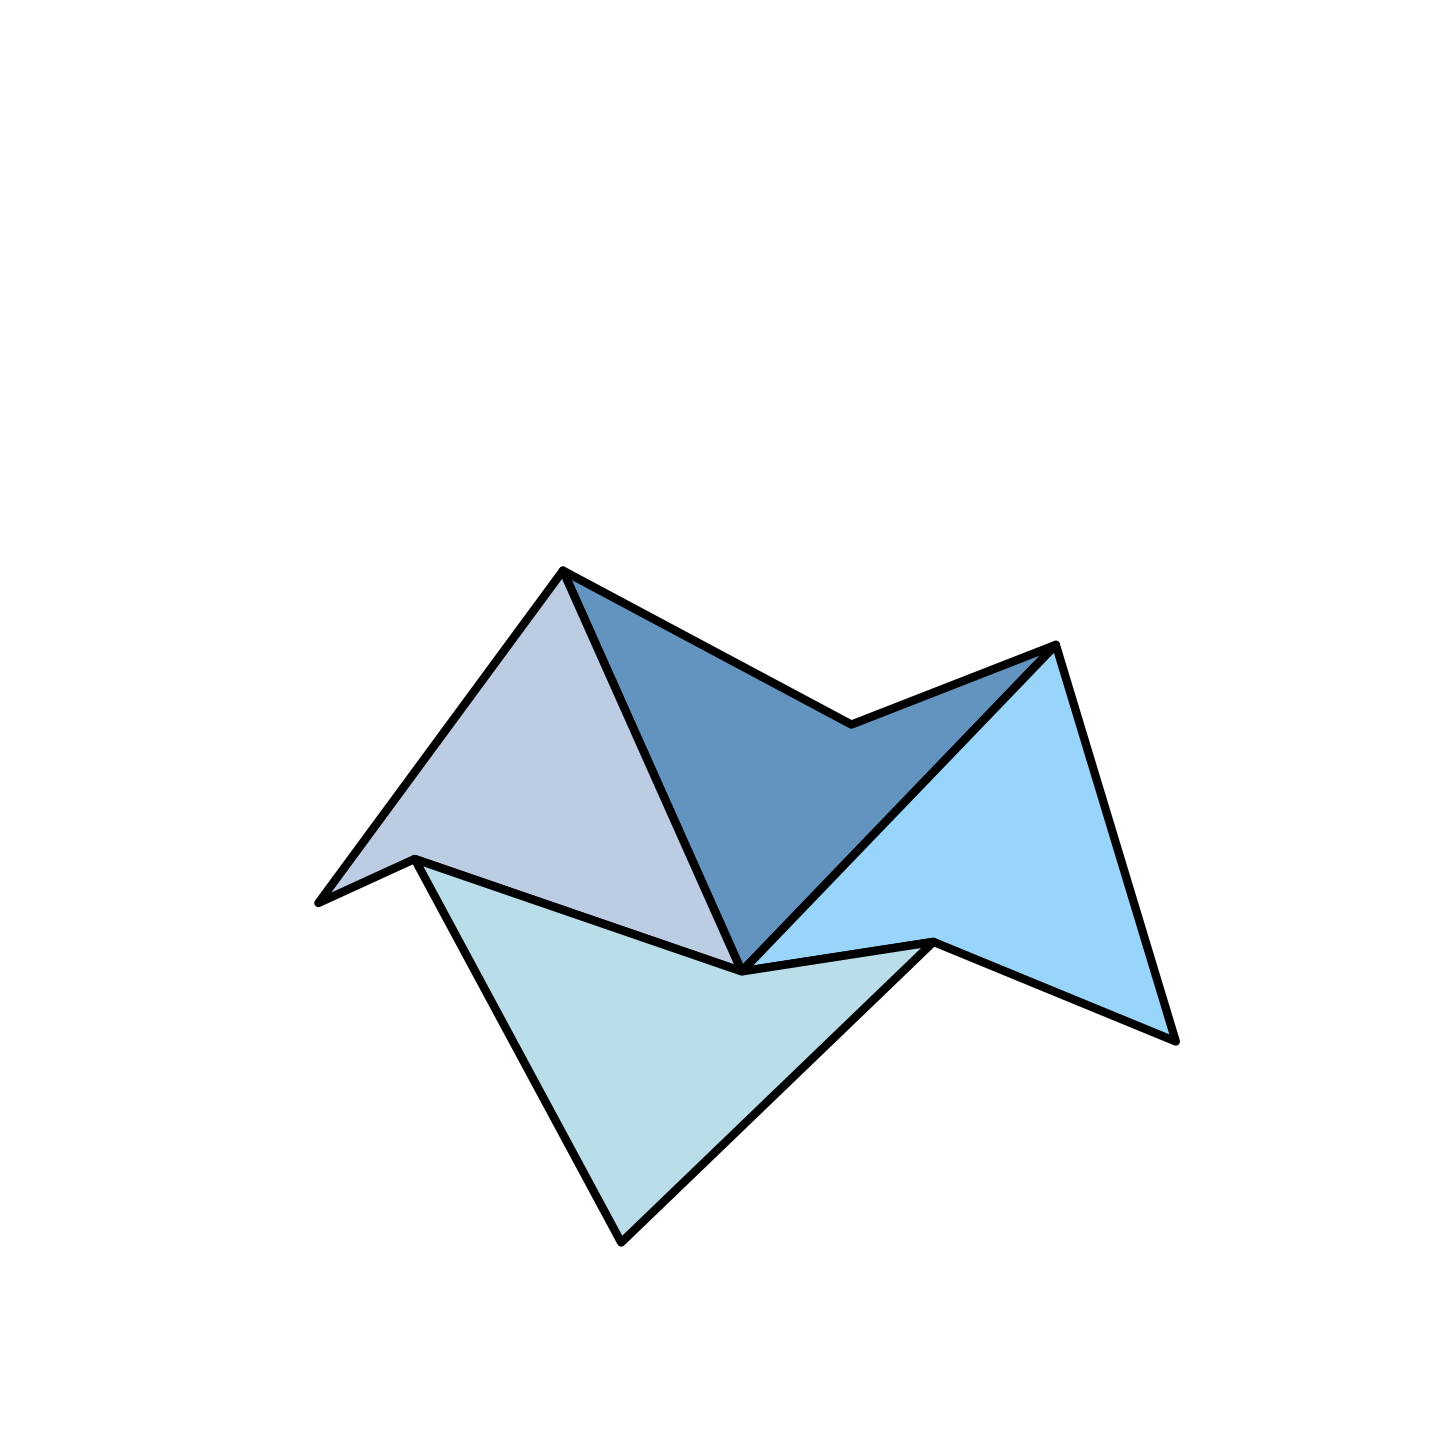
\includegraphics[width=\linewidth]{foto/origami_stage2.png}
    (b) Fase Setengah Lipat
  \end{minipage}\hfill
  \begin{minipage}{0.32\textwidth}
    \centering
    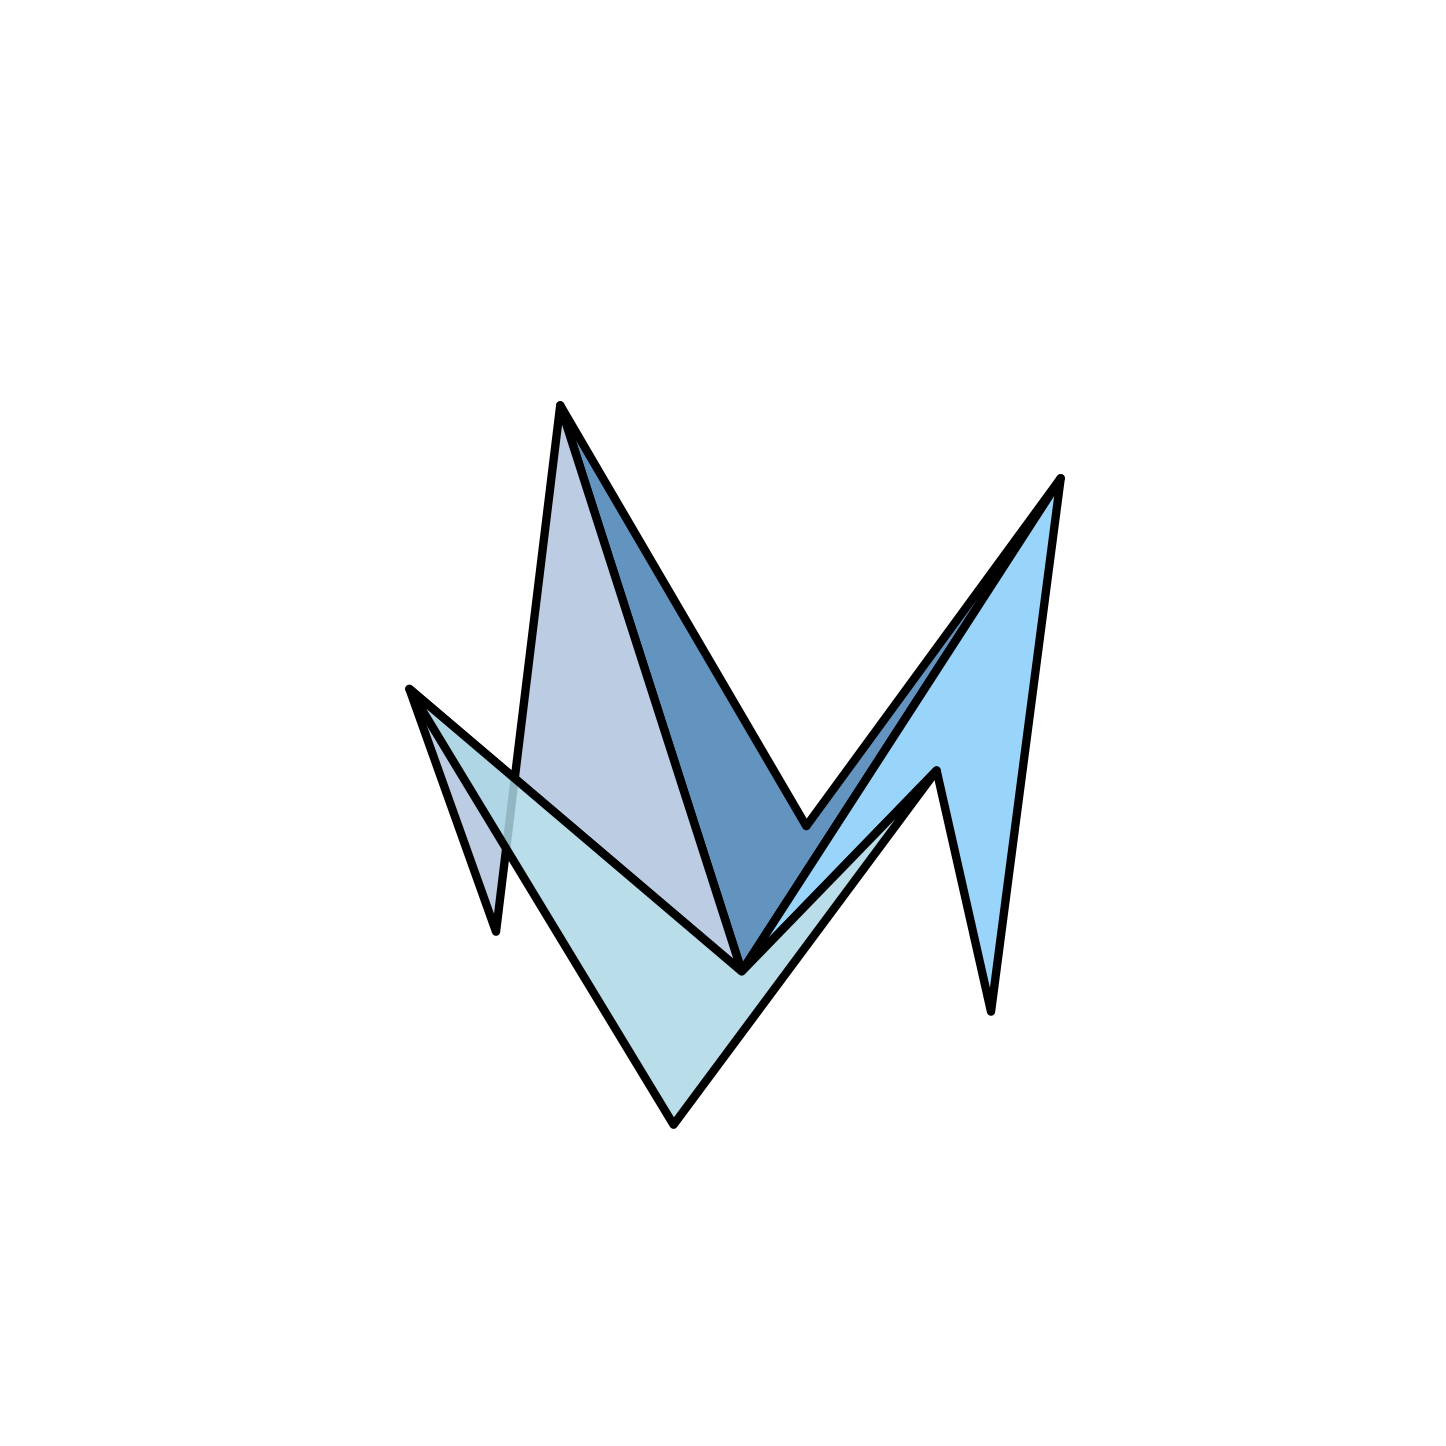
\includegraphics[width=\linewidth]{foto/origami_stage3.png}
    (c) Fase Lipat Kaku
  \end{minipage}
  \caption{Visualisasi 3D dari dinamika pelipatan kaku pada satu verteks origami dengan empat panel.}
  \label{fig:origami_stages}
\end{figure}

Analisis pergerakan kontinu tiga dimensi pada pelipatan kaku secara tradisional diselesaikan dengan mengalikan rantai matriks rotasi ortogonal khusus $SO(3)$ di setiap engsel. Representasi jaring lipatan origami menggunakan matriks ketetanggaan (\textit{adjacency matrix}) mampu memetakan seluruh matriks rotasi tersebut \parencite{ku2014realization}. Meskipun model rotasi $SO(3)$ ini sangat akurat, pengoperasiannya bersifat non-linear majemuk karena melibatkan fungsi trigonometri. Ketika skala sistem diperbesar untuk memodelkan \textit{origami metamaterials} dengan ribuan verteks, komputasi non-linear ini memicu beban latensi yang masif.

Menghadapi kompleksitas non-linear tersebut, disiplin geometri aljabar modern menawarkan sebuah alternatif fundamental melalui geometri tropikal. Geometri tropikal dibangun di atas struktur semiring min-plus (atau max-plus), di mana operasi penjumlahan dan perkalian polinomial klasik didekuantisasi menjadi operasi pencarian nilai minimum dan penjumlahan linear \parencite{mikhalkin2006tropical}. Transformasi ini secara esensial mereduksi kurva derajat tinggi menjadi suatu permukaan \textit{piecewise-affine} yang linier terpotong-potong secara lokal.

\begin{figure}[H]
  \centering
  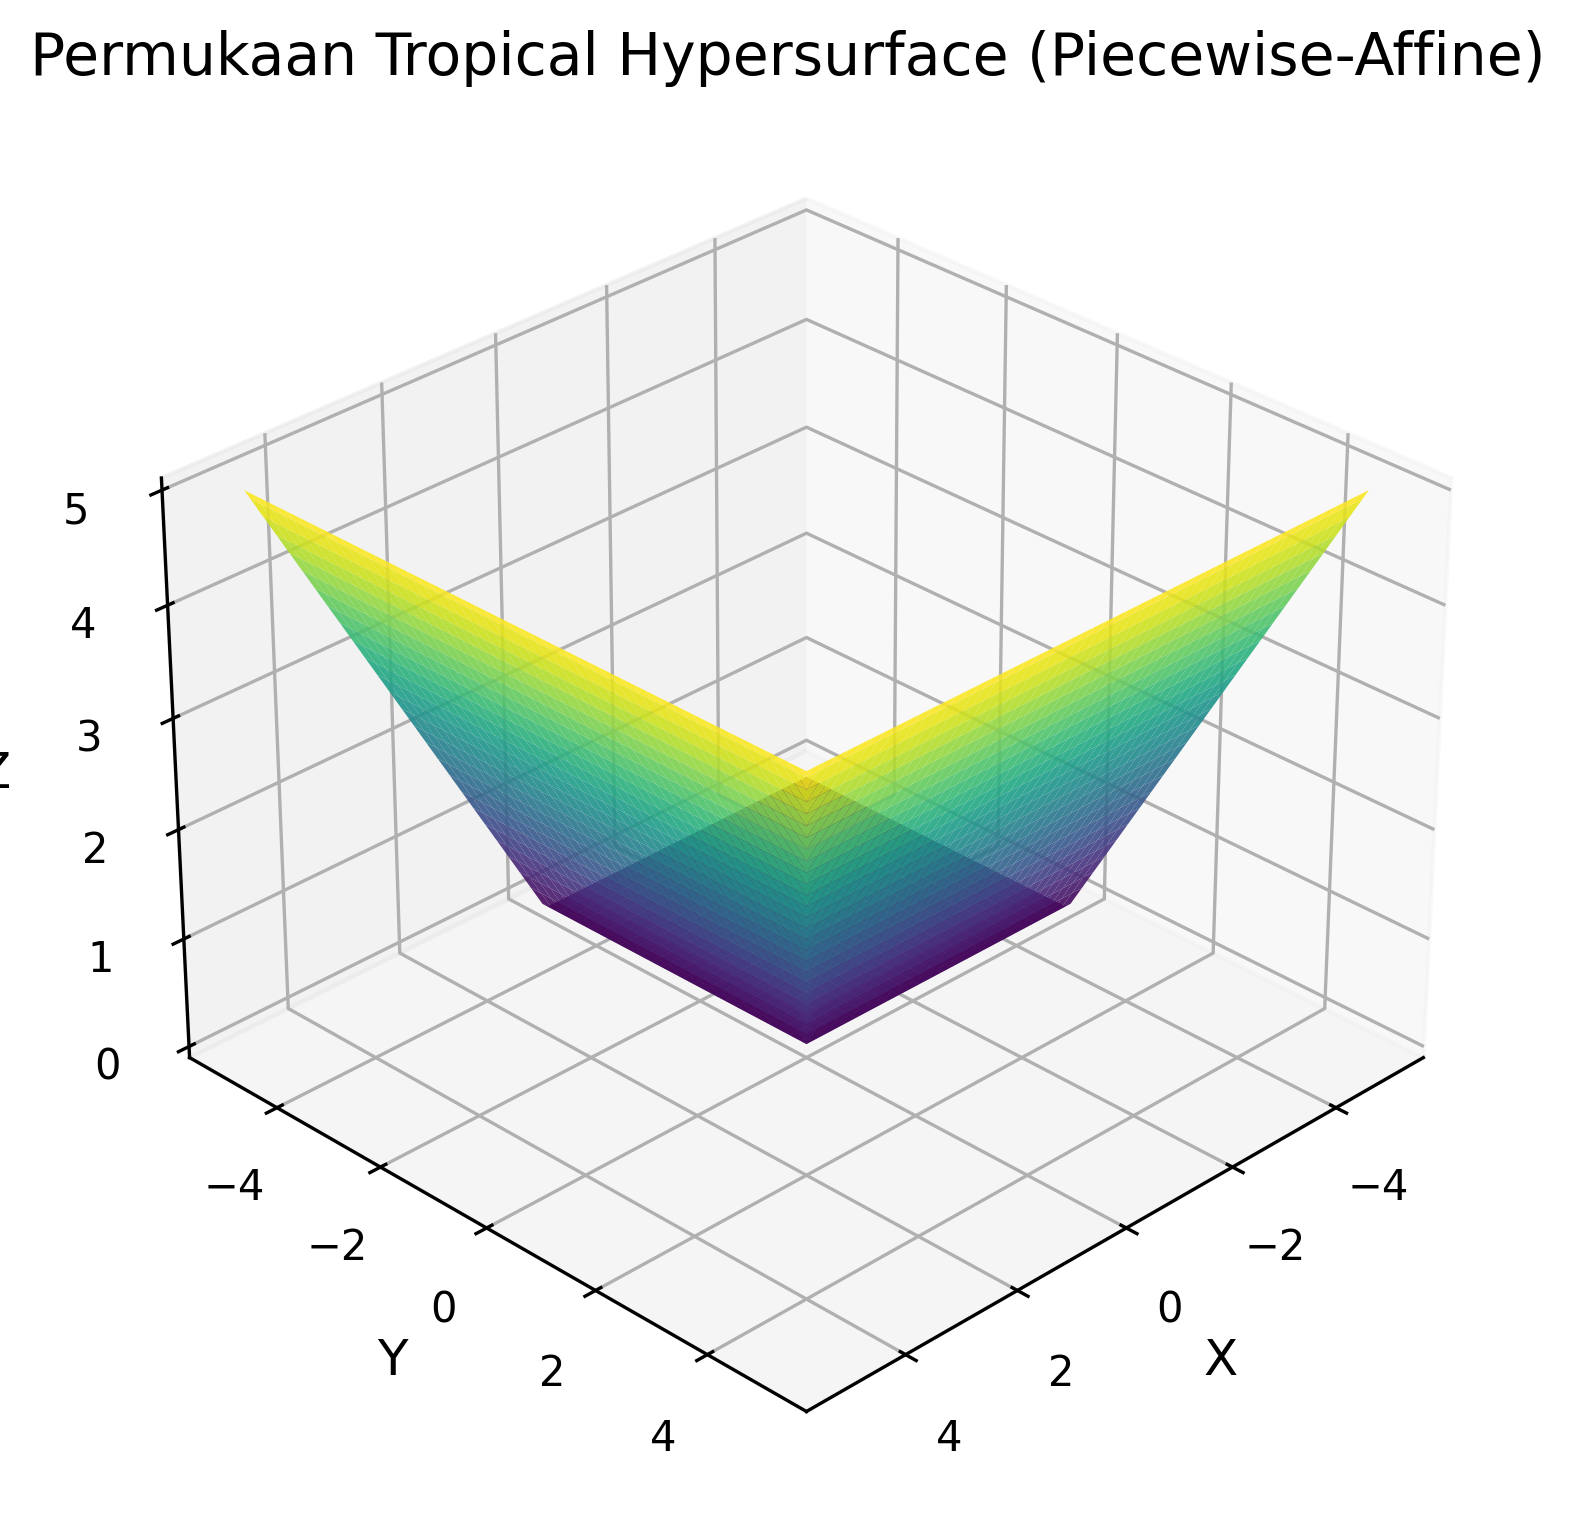
\includegraphics[width=0.7\linewidth]{foto/tropical_surface.png}
  \caption{Representasi permukaan 3D dari \textit{tropical hypersurface} yang mendemonstrasikan sifat konveks \textit{piecewise-affine}.}
  \label{fig:tropical_surface}
\end{figure}

Bentuk polinomial tropikal bermanifestasi sebagai kompleks polihedral (\textit{tropical hypersurfaces}) yang mempertahankan integritas geometrisnya melalui \textit{balancing condition} di setiap perpotongan sisinya \parencite{maclagan2015tropical}. Terdapat ekuivalensi struktural yang kuat antara \textit{balancing condition} tropikal dengan syarat kesetimbangan pelipatan pada origami, yakni Teorema Kawasaki dan Teorema Maekawa. Ekuivalensi parameter graf ini secara teoretis mengizinkan translasi model isometri lipatan konvensional ke dalam ruang metrik \textit{piecewise-affine} \parencite{gk2021origami, foster2020metric}.

Meskipun teori tropikal telah terbukti efisien dalam menyederhanakan komputasi dinamika jaringan saraf tiruan (\textit{neural networks}) \parencite{zhang2018tropical} dan memiliki fondasi yang sejalan dengan \textit{Gauge Theory} spasial \parencite{nekrasov2018geometry}, literatur matematika origami saat ini masih sepenuhnya bergantung pada operasi matriks kontinu. Hal ini menciptakan sebuah kesenjangan penelitian (\textit{research gap}) yang krusial, belum adanya formalisasi murni yang mensintesis isometri pelipatan kaku $SO(3)$ menjadi kerangka transformasi fungsi ruang tropikal diskrit yang berbiaya komputasi rendah.

Beranjak dari urgensi tersebut, riset tesis ini bertujuan merumuskan ulang pemodelan matematis \textit{rigid folding} origami secara ekuivalen ke dalam kerangka matriks aljabar tropikal \textit{piecewise-affine}.

\section{Rumusan Masalah}
Rumusan masalah dalam penelitian ini adalah sebagai berikut:
\begin{enumerate}
  \item Bagaimana memformulasikan Teorema Kawasaki dan Maekawa pada origami rigid secara ekuivalen sebagai fungsi ruang isometri tropikal \textit{piecewise-affine}?
  \item Bagaimana merumuskan isometri rotasi ortogonal ke dalam pembobotan polinomial lintasan \textit{adjacency graph} pada ruang modul min-plus?
\end{enumerate}

\section{Batasan Masalah}
Batasan masalah dalam penelitian ini adalah sebagai berikut:
\begin{enumerate}
  \item Penelitian ini difokuskan pada pelipatan datar (\textit{flat folding}) dan pelipatan kaku (\textit{rigid folding}) satu verteks (\textit{single vertex}).
  \item Pemodelan dilakukan menggunakan aljabar semiring min-plus dan fungsi \textit{piecewise-affine}.
\end{enumerate}

\section{Tujuan Penelitian}
Tujuan dari penelitian ini adalah sebagai berikut:
\begin{enumerate}
  \item Memformulasikan Teorema Kawasaki dan Maekawa pada origami rigid secara ekuivalen sebagai fungsi ruang isometri tropikal \textit{piecewise-affine}.
  \item Merumuskan isometri rotasi ortogonal ke dalam pembobotan polinomial lintasan \textit{adjacency graph} pada ruang modul min-plus.
\end{enumerate}

\section{Manfaat Penelitian}
Manfaat yang diharapkan dari penelitian ini adalah sebagai berikut:
\begin{enumerate}
  \item Secara teoritis, penelitian ini diharapkan dapat memberikan kontribusi pada pengembangan teori kombinatorik origami dalam kerangka geometri aljabar tropikal.
  \item Secara praktis, hasil penelitian ini diharapkan dapat membuka cara komputasional yang efisien untuk simulasi pelipatan material meta dan struktur \textit{deployable}.
  \item Sebagai bahan referensi untuk penelitian selanjutnya yang berkaitan dengan aplikasi fungsi \textit{piecewise-affine} pada permodelan benda fisik.
\end{enumerate}
